% Harus dimuat terlebih dahulu, digunakan agar file PDF memiliki format karakter yang benar.
% Untuk informasi lebih lanjut, lihat https://ctan.org/pkg/cmap.
\RequirePackage{cmap}

% Format dokumen sebagai paper konferensi menggunakan aturan IEEEtran terbaru (v1.8b).
% Untuk informasi lebih lanjut, lihat http://www.michaelshell.org/tex/ieeetran/.
\documentclass[a4paper, conference]{IEEEtran}

% Format encoding font dan input menjadi 8-bit UTF-8.
\usepackage[T1]{fontenc}
\usepackage[utf8]{inputenc}
\usepackage{amsmath}

% Digunakan untuk mengatur margin dokumen.
\usepackage{textcomp}

% Format bahasa menjadi bahasa indonesia dan inggris.
\usepackage[indonesian]{babel}

% Digunakan untuk tujuan demonstrasi.
\usepackage{mwe}

% Digunakan untuk menampilkan font dengan style yang lebih baik.
\usepackage[zerostyle=b,scaled=.75]{newtxtt}

% Digunakan untuk menampilkan tabel dengan style yang lebih baik.
\usepackage{booktabs}
\usepackage[table,xcdraw]{xcolor}
% Digunakan untuk menampilkan gambar pada dokumen.
\usepackage{graphicx}

% Digunakan untuk menampilkan potongan kode.
\usepackage{listings}
\lstset{
  basicstyle=\ttfamily,
  columns=fixed,
  basewidth=.5em,
  xleftmargin=0.5cm,
  captionpos=b
}

\usepackage{tabularx}
\usepackage{wrapfig}
% Digunakan agar backticks (`) dapat dirender pada PDF.
% Untuk informasi lebih lanjut, lihat https://tex.stackexchange.com/a/341057/9075.
\usepackage{upquote}

% Digunakan untuk menyeimbangkan bagian akhir dokumen dengan dua kolom.
\usepackage{balance}

% Kapitalisasi caption tabel
\usepackage{caption}
\captionsetup[table]{
    justification=centering, % Memusatkan caption
    labelsep=newline, % Memisahkan label "TABLE 1" dengan judul dengan baris baru
    textfont={sc}, % Membuat teks menjadi kapital
    labelfont={sc} % Membuat teks menjadi kapital
}


% Digunakan untuk menampilkan pustaka.
\usepackage[square,comma,numbers,sort&compress]{natbib}

% Untuk tabel
\usepackage{longtable}
\usepackage{array}

\usepackage{amsmath}
\usepackage{amssymb}


% Mengubah format ukuran teks pada natbib.
\renewcommand{\bibfont}{\normalfont\footnotesize}

% Jika melebihi 3 penulis dapat dilakukan linebreakend 
\makeatletter
\newcommand{\linebreakand}{%
  \end{@IEEEauthorhalign}
  \hfill\mbox{}\par
  \mbox{}\hfill\begin{@IEEEauthorhalign}
}
\makeatother

% Menambah nama penulis ketika menggunakan perintah \citet.
% Untuk informasi lebih lanjut, lihat https://tex.stackexchange.com/a/76075/9075.
\usepackage{etoolbox}
\makeatletter
\patchcmd{\NAT@test}{\else \NAT@nm}{\else \NAT@hyper@{\NAT@nm}}{}{}
\makeatother

% Digunakan untuk melakukan linewrap pada pustaka dengan url yang panjang
% jika terdapat hyphens
\usepackage[hyphens]{url}

% Digunakan untuk menambah hyperlink pada referensi.
\usepackage{hyperref}

% Menonaktifkan warna dan bookmark pada hyperref.
\hypersetup{hidelinks,
  colorlinks=true,
  allcolors=black,
  pdfstartview=Fit,
  breaklinks=true
}

% Digunakan untuk membenarkan hyperref pada gambar.
\usepackage[all]{hypcap}

% Digunakan untuk menampilkan beberapa gambar
\usepackage[caption=false,font=footnotesize]{subfig}

\usepackage{stfloats}
% nama
\newcommand{\name}{Azzam Wildan Maulana}
\newcommand{\authorname}{Maulana, Azzam Wildan}
\newcommand{\nickname}{Wildan}
\newcommand{\advisor}{Muhtadin, S.T., M.T.}
\newcommand{\coadvisor}{Ahmad Zaini, S.T., M.T.}

% identitas
\newcommand{\nrp}{5024 20 1010}
\newcommand{\advisornip}{19800603 200604 1 003}
\newcommand{\coadvisornip}{19750419 200212 1 003}
\newcommand{\email}{5024201010@student.its.ac.id}
\newcommand{\advisoremail}{muhtadin@te.its.ac.id}
\newcommand{\coadvisoremail}{zaini@te.its.ac.id}

% judul
\newcommand{\tatitle}{KALIBRASI KAMERA \emph{OMNIVISION} PADA \emph{MOBILE ROBOT} MENGGUNAKAN \emph{MACHINE LEARNING}}
\newcommand{\engtatitle}{\emph{OMNIVISION CALIBRATION ON MOBILE ROBOT USING MACHINE LEARNING}}

% tempat
\newcommand{\place}{Surabaya}

% jurusan
\newcommand{\studyprogram}{Teknik Komputer}
\newcommand{\engstudyprogram}{Computer Engineering}

% fakultas
\newcommand{\faculty}{Teknologi Elektro dan Informatika Cerdas}
\newcommand{\engfaculty}{Intelligence Electrical and Informatics Technology}

% singkatan fakultas
\newcommand{\facultyshort}{FTEIC}
\newcommand{\engfacultyshort}{ELECTICS}

% departemen
\newcommand{\department}{Teknik Komputer}
\newcommand{\engdepartment}{Computer Engineering}

% Tambahkan format tanda hubung yang benar di sini
\hyphenation{
  ro-ket
  me-ngem-bang-kan
  per-hi-tu-ngan
}


\begin{document}

% Ubah kalimat berikut sesuai dengan judul penelitian.
\title{\tatitle{}}

% Ubah kalimat-kalimat berikut sesuai dengan nama, institusi, alamat dan kontak penulis.
\author{
  \IEEEauthorblockN{\name{}}
  \IEEEauthorblockA{\textit{Departemen \studyprogram{}}\\
    \textit{Institut Teknologi Sepuluh Nopember}\\
    Surabaya, Indonesia 60111\\
    \email{}}

  \and
  \IEEEauthorblockN{\advisor{}}
  \IEEEauthorblockA{\textit{Departemen \studyprogram{}}\\
    \textit{Institut Teknologi Sepuluh Nopember}\\
    Surabaya, Indonesia 60111\\
    \advisoremail{}}

  \and
  \IEEEauthorblockN{\coadvisor{}}
  \IEEEauthorblockA{\textit{Departemen \studyprogram{}}\\
    \textit{Institut Teknologi Sepuluh Nopember}\\
    Surabaya, Indonesia 60111\\
    \coadvisoremail{}}
}

% Digunakan untuk menampilkan judul dan deskripsi penulis.
\maketitle

% Mengubah keterangan `Abstract` ke bahasa indonesia.
% Hapus bagian ini untuk mengembalikan ke format awal.
\renewcommand\abstractname{Abstrak}

\begin{abstract}

  % Ubah paragraf berikut sesuai dengan abstrak dari penelitian.
  Dalam Kompetisi Robot sepak bola beroda, tim IRIS mendapatkan 
prestasi terbaiknya yaitu menjuarai RoboCup peringkat 3. 
Dalam permainan, Robot IRIS menggunakan kamera omnivision untuk 
mendeteksi hal-hal pada lingkungan sekitar. Selama ini, kalibrasi 
pada kamera omnivision menggunakan regresi polinominal satu arah sehingga 
hasilnya kurang baik pada arah yang lainnya. Tugas Akhir ini mengusulkan 
untuk menggunakan metode yang lerbih kompleks yaitu menggunakan 
pendekatan Machine Learning. 

\end{abstract}

% Mengubah keterangan `Index terms` ke bahasa indonesia.
% Hapus bagian ini untuk mengembalikan ke format awal.
\renewcommand\IEEEkeywordsname{Kata kunci}

\begin{IEEEkeywords}

  % Ubah kata-kata berikut sesuai dengan kata kunci dari penelitian.
  Deep Learning

\end{IEEEkeywords}


% Ubah bagian berikut sesuai dengan konten-konten yang akan dimasukkan pada dokumen
% Ubah judul dan label berikut sesuai dengan yang diinginkan.
\section{Pendahuluan}
\label{sec:pendahuluan}

% Ubah paragraf-paragraf pada bagian ini sesuai dengan yang diinginkan.

There are three main parts of Mobile Robot, namely Sensor, Control, and Actuator. All the main parts are connected to each other. Sensor is used to detect the environment around the robot. Control is used to process the data from the sensor and decide the next action. Actuator is used to execute the action that has been decided by the control.  
 
There is a sensor for Mobile Robot that can sense 360 degree around the robot. The sensor is called Omnivision Camera. The use of Omnivision Camera give more benefits because it can grab the information around robot with only one capture. The basic concept of Omnivision Camera is to use a mirror to reflect the environment around the robot. The mirror is placed in front of the camera. The camera is placed in the middle of the mirror and projected 90 degree to the ground of Robot. Not only can sense the environment around the robot, the camera can also sense within 10m distance.
% Ubah judul dan label berikut sesuai dengan yang diinginkan.
\section{Tinjauan Pustaka}
\label{sec:tinjauanpustaka}

% Ubah bagian-bagian berikut dengan isi dari tinjauan pustaka
\subsection{Hasil penelitian/perancangan terdahulu}
Metode Regresi Polinomial adalah sebuah metode pendekatan terhadap data-data yang telah disediakan sebelumnya. Hasil keluaran dari metode Regresi Polinomial ini berupa rumusan matematika berdasarkan data-data yang telah disediakan. Regresi polinomial dapat bekerja secara efisien meskipun dengan model yang non-linear 
\citet{ref_regresi}.

\subsection{Teori/Konsep Dasar}

\subsubsection{Kamera \emph{Omnivision}}
\label{sec:omnivision}
\begin{figure}[ht]
    \centering
  
    % Ubah dengan nama file gambar dan ukuran yang akan digunakan
    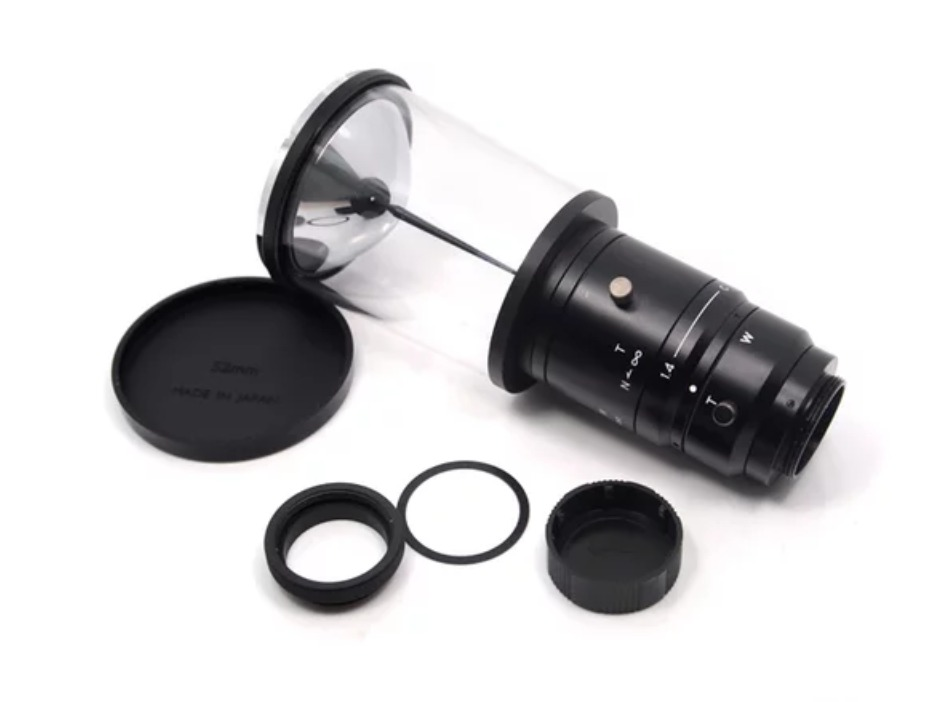
\includegraphics[width=8cm]{gambar/omnivisino2.jpeg}
  
    % Ubah dengan keterangan gambar yang diinginkan
    \caption{Kamera Omnivsion.}
    \label{fig:omnivision}
\end{figure}
Kamera \emph{omnivision} adalah sebuah kamera yang bisa melihat 360 derajat sekitar 
kamera tersebut \citet{ref_kamera_omni}. 
Jarak pandang kamera \emph{omnivision} tidak terbatas 
tergantung dari resolusi kamera itu sendiri dan 
konstruksi cerminnya. Pada dasarnya kamera \emph{omnivision} 
adalah kamera biasa yang ditembakkan ke sebuah cermin cembung 
sehingga pandangan kamera tersebut bisa ke segala arah. 

\subsubsection{Neural Network}
\label{sec:nn}
\begin{figure}[ht]
    \centering
  
    % Ubah dengan nama file gambar dan ukuran yang akan digunakan
    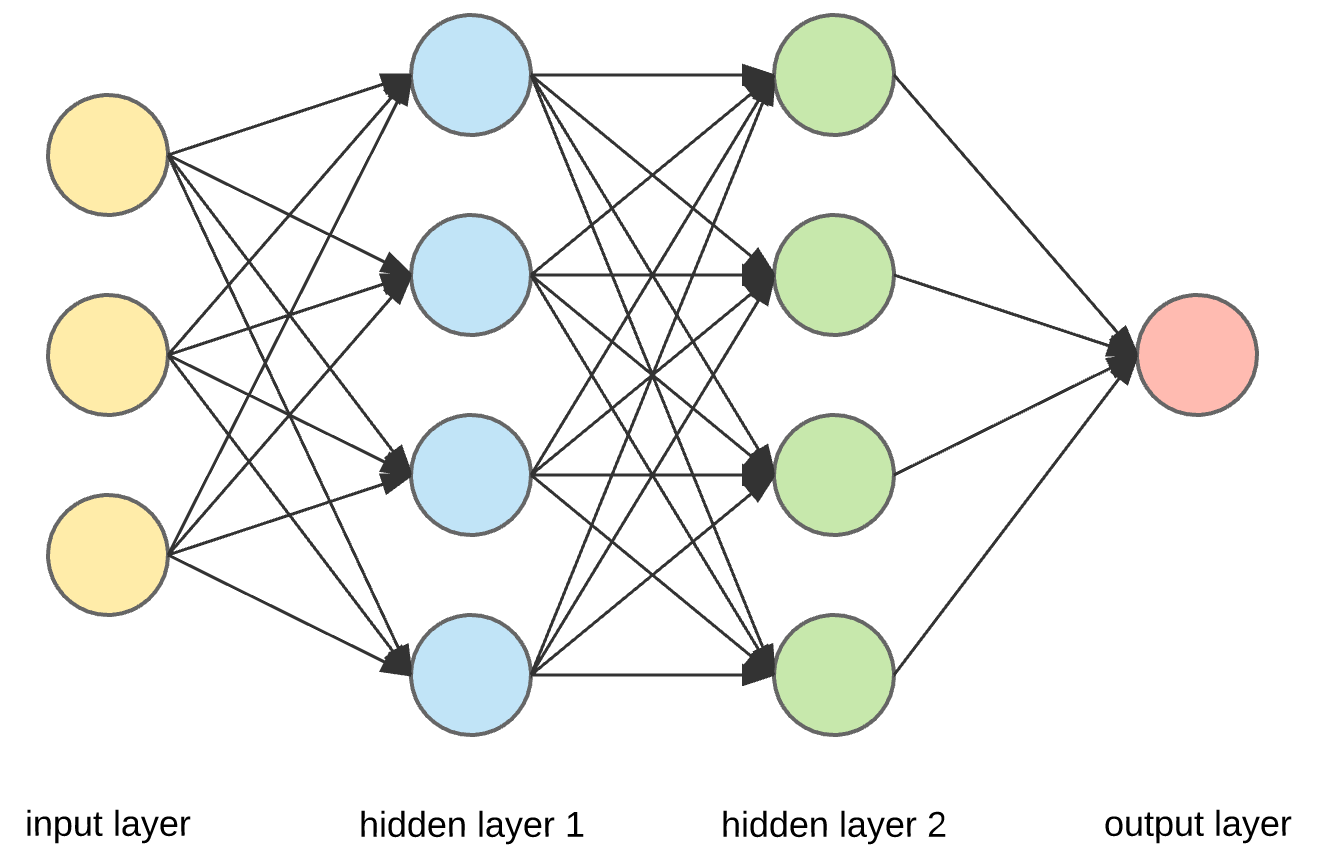
\includegraphics[width=8cm]{gambar/nn.png}
  
    % Ubah dengan keterangan gambar yang diinginkan
    \caption{Neural Network.}
    \label{fig:nn}
\end{figure}
\emph{Neural network} merupakan bagian dari Pembelajaran Mesin. 
\emph{Neural network} diciptakan untuk mengatasi masalah ketidaklinearan 
pada sebuah model \citet{ref_neural_network}. Pada dasarnya, 
\emph{Neural network} hanyalah sekumpulan \emph{Neuron} 
yang terhubung oleh sebuah \emph{Weight} dan \emph{Bias}. Selain 
\emph{Weight} dan \emph{Bias}, ada juga namanya \emph{forward propagation} 
menggunakan \emph{activation function} atau 
biasa disebut transfer function. Selain \emph{forward propagation},
 terdapat \emph{backward propagation} menggunakan \emph{loss function}. 

\subsubsection{\emph{Activation Function}}
\emph{Activation function} adalah sebuah fungsi yang digunakan untuk men-transfer 
data pada masing-masing layer pada \emph{Neural Network}. 
Dalam \emph{Neural Network}, \emph{Activation function} berperan sebagai 
\emph{forward propagation} yaitu perjalanan dari layer input menuju 
layer output. Beberapa \emph{activation Function} memiliki nilai 
saturasi biasanya bernilai 1 contohnya Sigmoid yang bernilai 
pada interval 0 sampai 1. Ada juga \emph{activation Function} lain yaitu 
tanh yang bernilai pada interval -1 sampai 1 \citet{ref_activation_function}.

\subsubsection{\emph{Loss Function}}
\emph{loss function} adalah bagian dari \emph{Neural Network} 
yang bertujuan untuk memberikan umpan balik 
pada model tentang baik atau buruknya fase \emph{training}. 
\emph{loss function} pada \emph{Neural Network} bekerja pada jalur 
\emph{Backward Propagation} yaitu dari layer output menuju layer input. 
Ada beberapa macam \emph{loss function} salah satunya adalah MSE 
(\emph{Mean Squared Error}). MSE \emph{loss function} lebih baik digunakan pada 
data dengan nilai fluktuasi yang rendah \citet{ref_loss_function}. 

Selain \emph{loss function}, ada sebuah teori lagi yaitu Optimizer. 
Optimizer adalah sebuah algoritma yang bisa digunakan untuk menentukan 
\emph{learning rate} sistem training. \emph{Learning rate} pada 
\emph{Neural Network} digunakan untuk mengatur seberapa cepat model 
akan konvergen terhadap data-datanya. 

\subsubsection{\emph{Mobile Robot}}
\label{sec:mobile_robot}
\begin{figure}[ht]
    \centering
  
    % Ubah dengan nama file gambar dan ukuran yang akan digunakan
    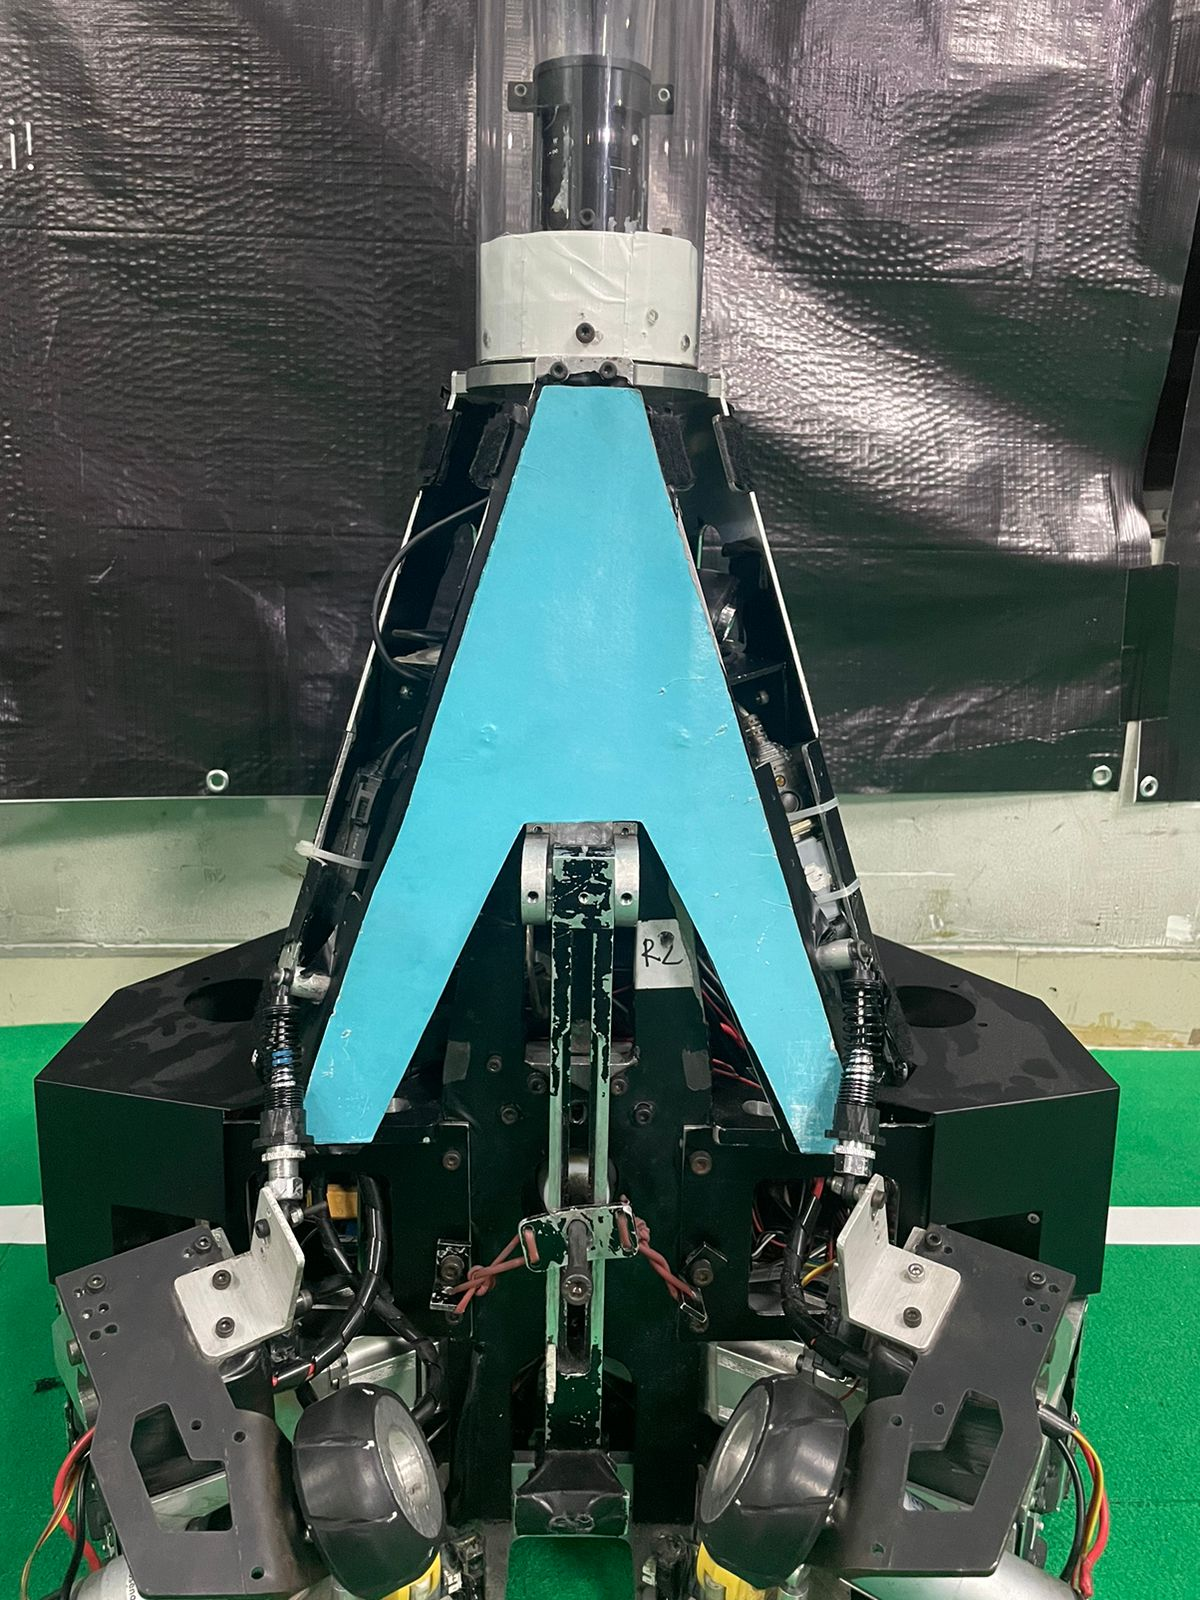
\includegraphics[width=6cm]{gambar/iris1.jpeg}
  
    % Ubah dengan keterangan gambar yang diinginkan
    \caption{Robot IRIS tampak depan.}
    \label{fig:mobile_robot}
\end{figure}
\emph{Mobile Robot} adalah sebuah robot yang didesain agar bisa bergerak 
atau berpindah tempat dengan mudah. Performa \emph{Mobile Robot} banyak 
dikhususkan pada sistem tracking, lokalisasi, dan algoritma. Ketiga 
hal tersebut berdasar pada kemampuan sensing yang baik \citet{ref_mobile_robot}. 
Pada umumnya, sensor yang digunakan adalah kamera baik itu kamera biasa 
maupun kamera \emph{omnivision}. Penggunaan kamera \emph{omnivision} dapat 
membuat robot melihat ke segala arah, Namun pre-processing datanya yang 
lebih sulit dibandingkan dengan kamera biasa.

\subsubsection{\emph{OpenCV}}
\label{sec:opencv}
\begin{figure}[ht]
    \centering
  
    % Ubah dengan nama file gambar dan ukuran yang akan digunakan
    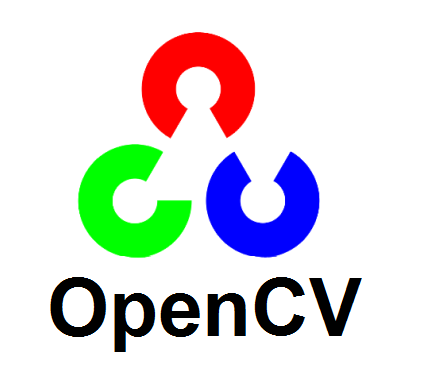
\includegraphics[width=8cm]{gambar/opencv.png}
  
    % Ubah dengan keterangan gambar yang diinginkan
    \caption{Logo OpenCV.}
    \label{fig:opencv}
\end{figure}
\emph{OpenCV} adalah library open-source yang dikembangkan oleh 
Intel dengan bahasa pemrograman C/C++. 
\emph{OpenCV} menyediakan banyak algoritma yang berhubungan dengan Visi 
Komputer \citet{ref_opencv}. OpenCV banyak digunakan untuk deteksi 
objek baik itu berdasarkan warna, bentuk, ukuran, dan lain lain 
sesuai kebutuhan program. 

\subsubsection{Robot Operating System}
\label{sec:ros}
\begin{figure}[ht]
    \centering
  
    % Ubah dengan nama file gambar dan ukuran yang akan digunakan
    
\includegraphics[width=8cm]{gambar/ros.png}
  
    % Ubah dengan keterangan gambar yang diinginkan
    \caption{Logo ROS.}
    \label{fig:ros}
\end{figure}
ROS atau \emph{Robot Operating System} adalah sebuah platform yang berdiri 
diatas 
Linux dan berguna untuk sinkronisasi bagian bagian dari 
robot \citet{ref_ros}. ROS banyak digunakan sebagai inti 
pemrosesan data dari sebuah robot mulai dari pemrosesan data sensor 
hingga menjadi data aktuator. ROS menyediakan konsep modular programming 
dengan metode publish/subscribe untuk IPC (\emph{Inter Process Communication}) nya. Selain memudahkan untuk 
transfer data antar proses, ROS juga menyediakan timer dengan scheduler 
default nya mengikuti Default Linux Scheduler yaitu Priority-based scheduler. 
Hal itu memungkinkan pengguna untuk mengatur prioritas masing-masing bagian 
dari robotnya. 

\subsubsection{Websocket}
Websocket adalah jenis protokol komunikasi berbasis protokol TCP (\emph{Transmission Control Protocol}). 
Protokol websocket membuat kedua pengirim dan menerima untuk selalu 
membuka socket nya agar bisa saling komunikasi. 
Dibandingkan dengan HTTP (\emph{Hypertext Transfer Transfer Protocol}), 
protokol Websocket memiliki 
latensi yang lebih baik \citet{ref_websocket}. Aplikasi 
websocket banyak digunakan untuk aplikasi obrolan (chat), game online,
 aplikasi yang membutuhkan data \emph{realtime}, dan masih banyak lainnya. 

% Ubah judul dan label berikut sesuai dengan yang diinginkan.
\section{Desain dan Implementasi}
\label{sec:desaindanimplementasi}

\subsection{Desain Sistem}
\label{subsec:desainsistem}

% Contoh input gambar pada kolom.
\begin{figure} [ht]
  \centering
  % Ubah sesuai dengan nama file gambar dan ukuran yang akan digunakan.
  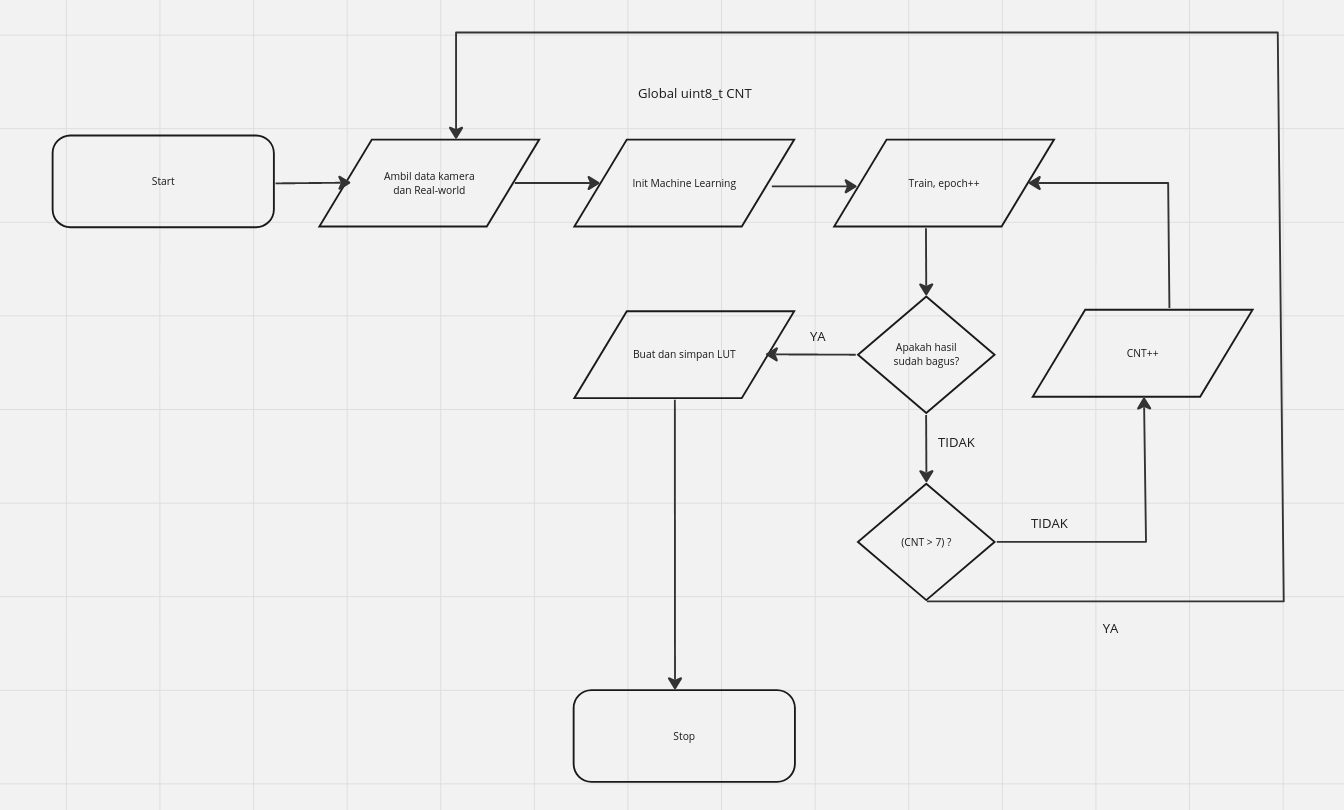
\includegraphics[width=0.4\textwidth]{gambar/desain_sistem.png}

  % Ubah sesuai dengan keterangan gambar yang diinginkan.
  \caption{Desain Sistem Kalibrasi.}
  \label{fig:desainsistem}
\end{figure}

Pada desain sistem yang digunakan, terdapat beberapa tahapan proses yang dilakukan. Tahapan tersebut adalah sebagai berikut:

\begin{enumerate}
  \item \textbf{Pengambilan Data}: Pada tahapan ini, data yang diambil adalah data koordinat titik pada kamera dan data koordinat titik pada dunia nyata.
  \item \textbf{Machine Learning}: Pada tahapan ini, data koordinat yang telah diambil akan dilakukan proses \emph{training} menggunakan metode \emph{Machine Learning}. Adapun metode yang digunakan adalah \emph{Neural Network}.
  \item \textbf{Pembuatan \emph{Lookup Table}}: Pada tahapan ini, hasil dari \emph{training} akan digunakan untuk membuat \emph{lookup table} yang akan digunakan untuk kalibrasi kamera. \emph{Lookup table} dibuat dengan mengunakan dua \emph{byte memory} untuk setiap koordinat titik pada kamera.
\end{enumerate}

\subsection{Implementasi pada Robot}
\label{subsec:implementasi}

Implementasi dari sistem kalibrasi kamera omnivision menggunakan \emph{Machine Learning} dilakukan melalui beberapa tahapan. Tahapan tersebut adalah sebagai berikut: 

\begin{enumerate}
  \item \textbf{\emph{Load Lookup Table}}: Pada tahapan ini, \emph{lookup table} yang telah dibuat akan dimuat ke dalam program dalam bentuk \emph{array}. 
  \item \textbf{Kalibrasi Kamera}: Pada tahapan ini, kamera akan diarahkan ke titik yang telah ditentukan. Kemudian, kamera akan mengambil gambar dan mengirimkan data koordinat titik ke program. Program akan mengubah data koordinat tersebut menjadi data koordinat yang benar berdasarkan \emph{lookup table}.
\end{enumerate}
% Ubah judul dan label berikut sesuai dengan yang diinginkan.
\section{Hasil dan Pembahasan}
\label{sec:hasildanpembahasan}

\subsection{Visualisasi Hasil Kalibrasi}
\label{sec:visualisasihasil} 

Visualisasi hasil kalibrasi dilakukan dengan cara data pada kamera dengan data pada lapangan. Hal itu dilakukan dengan cara memasukkan data pada kamera ke dalam \emph{Lookup Table} yang telah dibuat sebelumnya. Berikut adalah hasil visualisasi yang didapat. 

\begin{figure}[ht]
  \centering
  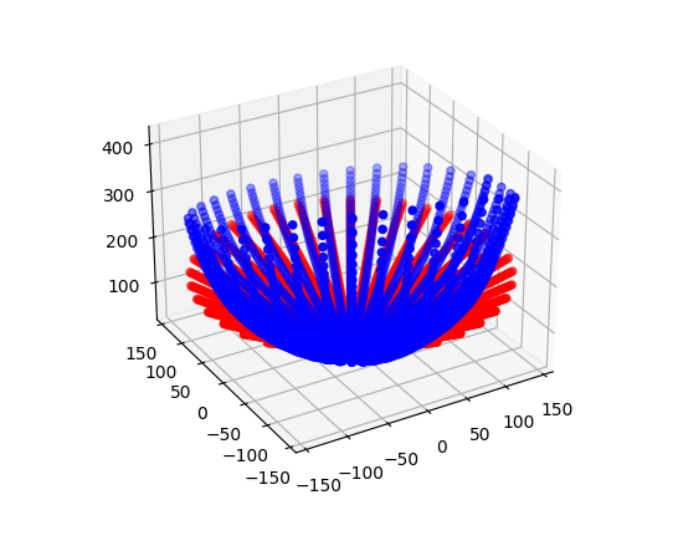
\includegraphics[width=8cm]{gambar/visual1.png}
  \caption{Visualisasi hasil kalibrasi.}
  \label{fig:hasilkalibrasi}
\end{figure}

Dari gambar tersebut, dapat dilihat bahwa data pada kamera yang digunakan tidak sepenuhnya diproyeksikan tegak lurus 90 derajat dengan lapangan. Hal itu terjadi karena kamera yang digunakan tidak terpasang dengan benar. 

\subsection{Skenario Pengujian Akurasi}
\label{sec:skenariopengujian}

Pengujian dilakukan dengan cara mendeteksi bola yang diam di lapangan dengan memutar robot pada posisinya sendiri. Hal itu membuat robot dapat melihat bola dari berbagai sudut. Pengujian dilakukan dengan mengambil data dari kamera omnivision yang telah terpasang pada robot lalu memroses data tersebut menggunakan \emph{Lookup Table} yang telah dibuat sebelumnya sehingga didapat koordinat bola pada lapangan. Berikut adalah skenario pengujian yang dilakukan: 

\begin{figure}[ht]
  \centering
  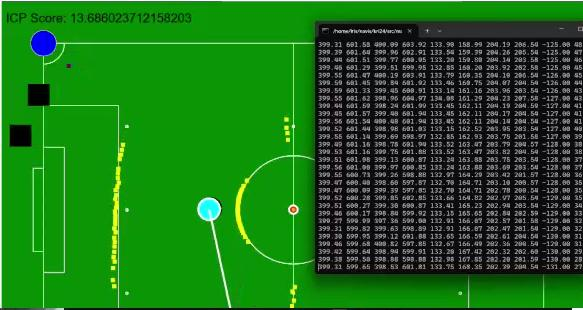
\includegraphics[width=8cm]{gambar/saat_putar_bola_2.jpeg}
  \caption{Skenario Pengujian.}
  \label{fig:skenariopengujian}
\end{figure}

Prosedur tersebut dilakukan pada jarak robot dengan bola pada lapangan yang berbeda-beda yaitu pada 120 cm, 200 cm, dan 285 cm. 

Adapun rumusan yang digunakan untuk menghitung posisi bola pada lapangan adalah sebagai berikut: 

\begin{equation}
  \begin{aligned}
    dx &= x\_bola\_cam - x\_center\_cam \\
    dy &= y\_center\_cam - y\_bola\_cam \\
    r\_bola\_cam &= \sqrt{dx^2 + dy^2} \\
    \theta\_bola\_cam &= \arctan(\frac{dy}{dx}) \\
    index &= \theta\_bola\_cam \times r\_max + r\_bola\_cam \\ 
    r\_bola\_lap &= r\_lookup[index] \\
    \theta\_bola\_lap &= \theta\_bola\_cam + robot\_pose\_\theta - 90 \\
    x\_bola &= robot\_pose\_x + r\_bola\_lap \times \cos(\theta\_bola\_lap) \\
    y\_bola &= robot\_pose\_y + r\_bola\_lap \times \sin(\theta\_bola\_lap) \\
  \end{aligned}
\end{equation}

\subsection{Evaluasi Pengujian Akurasi}
\label{sec:analisispengujian}

Dari pengujian yang telah dilakukan, didapat data sebagai berikut:

% Contoh pembuatan tabel
\begin{table}[htbp]
  \caption{Hasil Pengujian Posisi Bola pada Lapangan dengan Jarak 120 cm.}
  \begin{center}
    \begin{tabular}{|c|c|c|}
      \hline
    \rowcolor[HTML]{C0C0C0}
  \textbf{Sudut Robot ke Bola} & \textbf{Posisi Bola X} & \textbf{Posisi Bola Y} \\
  \hline

  0 deg            & 407.74 cm                & 596.67 cm            \\
  30 deg           & 409.41 cm                & 600.3 cm            \\
  60 deg           & 409.65 cm                & 600.54 cm            \\
  90 deg           & 407.52 cm                & 598.2 cm           \\
  120 deg           & 407.18 cm                & 600.07 cm           \\
  150 deg           & 409.98 cm                & 598.35 cm           \\
  180 deg           & 410.66 cm                & 593.41 cm           \\
  210 deg           & 410.84 cm                & 590.28 cm           \\
  240 deg           & 410.01 cm                & 590.8 cm           \\
  270 deg           & 409.9 cm                & 594.28 cm           \\
  300 deg           & 408.91 cm                & 590.14 cm           \\
  330 deg           & 408.8 cm                & 591.57 cm           \\
  \hline
\end{tabular}
\end{center}
\end{table}

\begin{table}[htbp]
  \caption{Hasil Pengujian Posisi Bola pada Lapangan dengan Jarak 200 cm.}
  \begin{center}

  \begin{tabular}{|c|c|c|}
  \hline
  \rowcolor[HTML]{C0C0C0}
  \textbf{Sudut Robot ke Bola} & \textbf{Posisi Bola X} & \textbf{Posisi Bola Y} \\
  \hline
  0 deg            & 406.44 cm                & 613.13 cm            \\
  30 deg           & 411.09 cm                & 624.66 cm            \\
  60 deg           & 416.39 cm                & 627.02 cm            \\
  90 deg           & 411.55 cm                & 625.85 cm           \\
  120 deg           & 408.85 cm                & 620.01 cm           \\
  150 deg           & 414.2 cm                & 611.7 cm           \\
  180 deg           & 415.12 cm                & 601.25 cm           \\
  210 deg           & 412.78 cm                & 592.09 cm           \\
  240 deg           & 410.77 cm                & 594.57 cm           \\
  270 deg           & 409.66 cm                & 598.43 cm           \\
  300 deg           & 407.92 cm                & 599.03 cm           \\
  330 deg           & 406.29 cm                & 602.72 cm           \\
  \hline
\end{tabular}
\end{center}
\end{table}

\begin{table}[htbp]
\caption{Hasil Pengujian Posisi Bola pada Lapangan dengan Jarak 285 cm.}
\begin{center}
  
\begin{tabular}{|c|c|c|}
  \hline
  \rowcolor[HTML]{C0C0C0}
  \textbf{Sudut Robot ke Bola} & \textbf{Posisi Bola X} & \textbf{Posisi Bola Y} \\
  \hline
  0 deg            & 380.98 cm                & 593.81 cm            \\
  30 deg           & 382.14 cm                & 594.49 cm            \\
  60 deg           & 383.41 cm                & 607.18 cm            \\
  90 deg           & 392.49 cm                & 604.67 cm           \\
  120 deg           & 390.32 cm                & 606.04 cm           \\
  150 deg           & 391.43 cm                & 598.47 cm           \\
  180 deg           & 387.17 cm                & 587.89 cm           \\
  210 deg           & 390.16 cm                & 577.15 cm           \\
  240 deg           & 389.67 cm                & 585.82 cm           \\
  270 deg           & 389.38 cm                & 590.31 cm           \\
  300 deg           & 382.61 cm                & 593.25 cm           \\
  330 deg           & 380.73 cm                & 589.31 cm           \\
  \hline
\end{tabular}
\end{center}
\end{table}


Dari tabel tersebut didapat standar deviasi pada data posisi bola pada lapangan dengan jarak 120 cm adalah 1.26 cm dan 4.11 cm untuk posisi bola x dan y. Sedangkan pada jarak 200 cm didapat standar deviasi 3.28 cm dan 12.80 cm untuk posisi bola x dan y. Pada jarak 285 cm didapat standar deviasi 4.40 cm dan 8.92 cm untuk posisi bola x dan y. 

Dari hasil tersebut dapat disimpulkan bahwa sistem kalibrasi yang telah dibuat dapat mendeteksi posisi bola pada lapangan dengan baik. Bola tidak tepat berada di tengah lapangan bisa disebabkan oleh beberapa faktor. Adapun beberapa faktor penyebabnya adalah ketidaktepatan posisi bola pada dunia aslinya, ketidaktepatan posisi robot pada dunia aslinya, dan ketidaktepatan orientasi robot pada dunia aslinya. Karena pada dasarnya sesuai dengan rumus \textbf{4.1}, posisi bola pada lapangan juga ditentukan oleh posisi robot pada lapangan. 

\subsection{Skenario Pengujian Akurasi Kedua}
\label{sec:skenariopengujian2}

Pengujian akurasi kedua adalah dengan cara membandingkan hasil kalibrasi baru dengan kalibrasi lama yang masih menggunakan algoritma \emph{regresi polynomial}. Pengujian dilakukan dengan cara yang sama seperti pengujian akurasi sebelumnya. Namun, proses perhitungannya menggunakan algoritma \emph{regresi polynomial}. 

\subsection{Evaluasi Pengujian Akurasi Kedua}
\label{sec:analisispengujian2}
\begin{table}[htbp]

\caption{Hasil Pengujian Posisi Bola pada Lapangan dengan Jarak 120 cm menggunakan Kalibrasi Lama.}
\begin{center}
  

\begin{tabular}{|c|c|c|}
  \hline
  \rowcolor[HTML]{C0C0C0}
  \textbf{Sudut Robot ke Bola} & \textbf{Posisi Bola X} & \textbf{Posisi Bola Y} \\
  \hline
  0 deg            & 370.18 cm                & 576.31 cm            \\
  30 deg           & 376.24 cm                & 585.42 cm            \\
  60 deg           & 383.91 cm                & 597.98 cm            \\
  90 deg           & 392.99 cm                & 605.67 cm           \\
  120 deg           & 390.23 cm                & 610.94 cm           \\
  150 deg           & 400.49 cm                & 598.89 cm           \\
  180 deg           & 385.97 cm                & 582.89 cm           \\
  210 deg           & 398.61 cm                & 577.15 cm           \\
  240 deg           & 390.76 cm                & 585.02 cm           \\
  270 deg           & 386.32 cm                & 588.91 cm           \\
  300 deg           & 378.69 cm                & 585.55 cm           \\
  330 deg           & 370.32 cm                & 579.11 cm           \\
  \hline
\end{tabular}
\end{center}
\end{table}

Dari data tersebut dapat dilihat bahwa standar deviasi pada data posisi bola pada lapangan dengan jarak 120 cm menggunakan kalibrasi lama adalah 10.01 cm dan 11.32 cm untuk posisi bola x dan y. Sedangkan pada kalibrasi baru standar deviasi 1.26 cm dan 4.11 cm untuk posisi bola x dan y. Dapat dilihat bahwa kalibrasi baru lebih baik dibandingkan dengan kalibrasi lama. Hal itu terjadi karena pemasangan kamera pada robot yang tidak tepat sehingga menyebabkan hasil kalibrasi lama menjadi tidak akurat. Ketidakakuratan tersebut terjadi karena kalibrasi lama hanya menggunakan satu arah saja sebagai referensi untuk model regresi polynomial. Sedangkan, pada kenyataannya rumus model untuk masing-masing arah kamera akan selalu berbeda.  

\subsection{Skenario Pengujian Kecepatan Komputasi}
\label{sec:analisispengujian}

Pengujian dilakukan dengan cara membandingkan apakah sistem kalibrasi baru lebih cepat dibandingkan menggunakan sistem kalibrasi lama. Pengujian dilakukan dengan cara mencatat waktu setelah kalibrasi lalu menguranginya dengan waktu sebelum kalibrasi. Sehingga bisa didapat perkiraan waktu lamanya sistem melakukan proses perhitungan untuk melakukan kalibrasi. Berikut rumus yang digunakan untuk menghitung waktu delay: 

\begin{equation}
  \begin{aligned}
    delay\_time &= waktu1 - waktu0 \\ 
  \end{aligned}
\end{equation}

Dimana $waktu1$ adalah waktu setelah kalibrasi dan $waktu0$ adalah waktu sebelum kalibrasi.


\subsection{Evaluasi Pengujian Kecepatan Komputasi}
\label{sec:analisispengujian}

Dari pengujian yang telah dilakukan, didapat data sebagai berikut: 

\begin{table}{|c|c|c|}
  \caption{Hasil Pengujian Perbedaan Kecepatan Komputasi}
\begin{center}
  

\begin{tabular}{|c|c|c|}
  \hline
  \rowcolor[HTML]{C0C0C0}
  \textbf{Iterasi ke-} & \textbf{Waktu Kalibrasi Baru} & \textbf{Waktu Kalibrasi lama} \\
  \hline
  0            & 119 ns                & 176 ns            \\
  1           & 76 ns                & 86 ns            \\
  2           & 25 ns                & 107 ns            \\
  3           & 31 ns                & 90 ns           \\
  4           & 32 ns                & 88 ns           \\
  5           & 36 ns                & 87 ns           \\
  6           & 37 ns                & 88 ns           \\
  7           & 34 ns                & 93 ns           \\
  8           & 37 ns                & 89 ns           \\
  9           & 35 ns                & 90 ns           \\
  \hline
\end{tabular}
\end{center}
\end{table}

Dari grafik tersebut dapat dilihat bahwa sistem kalibrasi baru lebih cepat 53.2 ns dibandingkan dengan sistem kalibrasi lama. Dengan rata-rata Kalibrasi baru membutuhkan waktu 46.2 ns sedangkan kalibrasi lama membutuhkan waktu 99.4 ns. Hal tersebut disebabkan karena sistem kalibrasi baru hanya menggunakan \emph{Lookup Table} yang berisi data kalibrasi kamera. Sedangkan sistem kalibrasi lama menggunakan algoritma \emph{regresi polynomial} yang membutuhkan waktu lebih lama.
% Ubah judul dan label berikut sesuai dengan yang diinginkan.
\section{Kesimpulan}
\label{sec:kesimpulan}

% Ubah paragraf-paragraf pada bagian ini sesuai dengan yang diinginkan.

Dari hasil penelitian yang telah dilakukan, dapat disimpulkan bahwa metode kalibrasi kamera omnivision menggunakan \emph{Machine Learning} lebih baik daripada metode kalibrasi kamera omnivision menggunakan regresi polinomial. Hal ini dapat dilihat dari kemampuan metode kalibrasi kamera omnivision menggunakan \emph{Machine Learning} yang dapat meng-kalibrasi kamera omnivision pada semua arah. Sedangkan metode kalibrasi kamera omnivision menggunakan regresi polinomial hanya dapat meng-kalibrasi kamera omnivision pada satu arah saja. Selain itu, metode kalibrasi kamera omnivision menggunakan \emph{Machine Learning} juga membutuhkan waktu eksekusi yang lebih singkat daripada metode kalibrasi kamera omnivision menggunakan regresi polinomial. 
% Ucapan terima kasih jika ada
% \section{Ucapan Terima Kasih}
\label{sec:ucapanterimakasih}

Penulis mengucapkan terima kasih kepada Kementerian Riset, Teknologi, dan Pendidikan Tinggi Republik Indonesia atas \lipsum[1]

% Menampilkan daftar pustaka dengan format IEEE
\bibliographystyle{IEEEtranN}
\bibliography{pustaka/pustaka.bib}

% Menyeimbangkan bagian akhir di kedua kolom
\balance

\end{document}
